\documentclass[11pt,a4paper]{article}

\usepackage[utf8]{inputenc}
\usepackage[T1]{fontenc}
\usepackage[margin=2.4cm]{geometry}
\usepackage{microtype}
\usepackage{amsmath,amssymb}
\usepackage{graphicx}
% Resolve figures whether you run pdflatex from repo root (\path{figures/}) or from \path{reports/} (\path{../figures/}); keep a copy under \path{reports/figures/} for submissions.
\graphicspath{{figures/}{../figures/}}
\usepackage{booktabs}
\usepackage{hyperref}
\usepackage{url}
\usepackage{listings}
\usepackage[table]{xcolor}
\usepackage{tabularx}
\usepackage{enumitem}
\usepackage{tikz}
\usetikzlibrary{arrows.meta,positioning,shapes.multipart}
\definecolor{tblhead}{RGB}{214,227,248}
\definecolor{tblstripe}{RGB}{245,248,255}

\hypersetup{colorlinks=true,linkcolor=blue!50!black,citecolor=blue!50!black,urlcolor=blue!50!black}

% Softer line-breaking (reduces overfull boxes on long technical phrases).
\setlength{\emergencystretch}{2.5em}

\lstset{basicstyle=\ttfamily\footnotesize,breaklines=true,frame=single,columns=fullflexible,keepspaces=true}

% TOC: only \section lines (no \subsection) so the list fits on one page; use optional short titles on long headings.
\setcounter{tocdepth}{1}

\title{Technical Report:\\Recovering Cyber-Security Domain Knowledge\\
\large LoRA, Prompt Profiles, Dual-Mode RAG, and Multi-Benchmark Evaluation\\
\normalsize Generative AI --- Spring 2026}
\author{%
\begin{tabular}{c}
Farit Sharafutdinov \quad and \quad Grigorii Belayev\\[0.65em]
{\small Instructor: Bader Rasheed}%
\end{tabular}%
}
\date{\today}

\begin{document}
\maketitle

\begin{abstract}
We present a reproducible research stack for measuring \emph{over-refusal} on cyber-security instruction prompts and for comparing mitigation strategies: dual-mode offline RAG (TF--IDF and dense FAISS), prompt-profile ablations, and LoRA/QLoRA training on the same inference path as evaluation.
This document emphasizes \textbf{theoretical grounding} (low-rank adaptation geometry, sparse and dense retrieval statistics, known failure modes of long-context usage) and an \textbf{honest empirical split}: a \emph{development} configuration (small chat LM, fast iteration) versus the \emph{production} target (Llama-3-8B-Instruct in 4-bit), showing that the \textbf{pipeline} is sound while headline metrics depend strongly on backbone scale and decoding budget.
\textbf{Scope note:} we measure refusal \emph{rates} and uncertainty; we do not yet run a large gold adjudication separating appropriate refusals from false refusals on benign defensive tasks---that would be the next step if the claim is sharpened beyond stack validation.
\end{abstract}

\noindent\textbf{Repository.} \url{https://github.com/FaritSharafutdinov/Recovering-Cyber-Security-Domain-Knowledge}

\vspace{-0.4\baselineskip}
\begingroup
\small
\setlength{\parskip}{0pt plus 0.1pt}
\tableofcontents
\endgroup
\newpage

%==============================================================================
\section[Introduction]{Introduction and goals}
%==============================================================================

Aligned instruction-tuned LLMs trade off harmful completions against refusals; cyber-security education and defensive workflows sit uncomfortably near offensive lexical priors.
We build tooling to (i)~measure refusals with uncertainty, (ii)~isolate prompt effects, (iii)~inject retrieved evidence without paid judges, and (iv)~adapt with parameter-efficient fine-tuning---all with fixed integer query IDs for paired statistics.

\paragraph{Contributions.}
Farit Sharafutdinov: dataset/corpus direction, LoRA training pipeline, experiments.
Grigorii Belayev: evaluation protocol, inference/evaluation CLIs, orchestration and reporting.

%==============================================================================
\section[System scope]{System scope (condensed)}
\label{sec:inventory}
%==============================================================================

The repository is a \textbf{scripted laboratory}: \texttt{scripts/inference.py} and \texttt{scripts/train.py} for any Hugging Face causal LM (defaults to TinyLlama in code; Llama-3-8B 4-bit recommended for course-grade results); \texttt{retrieval\_augment\_queries.py} for TF--IDF or FAISS-augmented prompts; \texttt{build\_rag\_index.py} for dense indices; builders for MMLU/CTF subsets; \texttt{eval\_*} and \texttt{analyze\_trigger\_tokens.py} for metrics; \texttt{run\_experiment\_suite.py} and \texttt{run\_full\_report\_pipeline.py} as orchestrators; \texttt{smoke\_test.py} as a CI gate; manifests under \texttt{configs/}.
\texttt{STRUCTURE.md} is the authoritative file index.
Section~\ref{sec:report-map} and Table~\ref{tab:report-map} map orchestrators to \path{outputs/} paths and the Markdown or \LaTeX{} reports reviewers should open first.

\begin{figure}[ht]
\centering
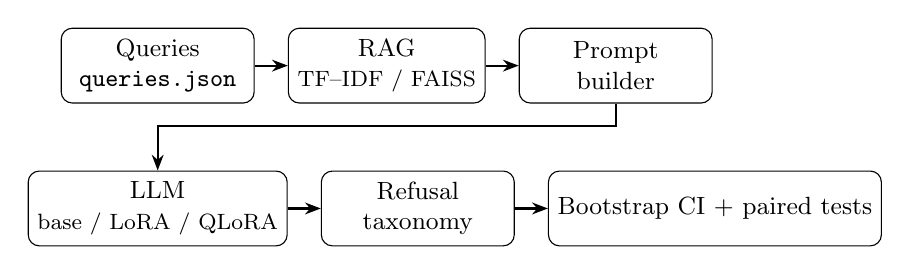
\begin{tikzpicture}[
  font=\small,
  box/.style={rectangle, draw, rounded corners, align=center, minimum width=2.45cm, minimum height=0.95cm},
  arrow/.style={-{Stealth[length=2mm]}, thick}
]
% First row: queries $\rightarrow$ RAG $\rightarrow$ prompt construction
\node[box] (q) {Queries\\\texttt{queries.json}};
\node[box, right=0.42cm of q] (rag) {RAG\\\footnotesize TF--IDF / FAISS};
\node[box, right=0.42cm of rag] (pb) {Prompt\\builder};
% Second row: LM $\rightarrow$ labels $\rightarrow$ uncertainty
\node[box, below=0.85cm of q] (llm) {LLM\\\footnotesize base / LoRA / QLoRA};
\node[box, right=0.42cm of llm] (cls) {Refusal\\taxonomy};
\node[box, right=0.42cm of cls] (bs) {Bootstrap CI + paired tests};
\draw[arrow] (q) -- (rag);
\draw[arrow] (rag) -- (pb);
\draw[arrow] (pb.south) -- ++(0,-0.28) -| (llm.north);
\draw[arrow] (llm) -- (cls);
\draw[arrow] (cls) -- (bs);
\end{tikzpicture}
\caption{End-to-end evaluation architecture: retrieval augments the prompt; the LM produces responses; refusal labels (manual or lexical) feed bootstrap and paired analyses.}
\label{fig:arch}
\end{figure}

%==============================================================================
\section{Data assets}
%==============================================================================

\texttt{queries.json} (50 IDs), \texttt{baseline\_outputs.json}, expert \texttt{baseline\_refusal\_labels.json}, \texttt{query\_tiers.json}, \texttt{trigger\_tokens.json}, \texttt{rag\_corpus.json} (optional JSONL), \texttt{prompt\_profiles.json}, \texttt{general\_capability\_mcq.json}; generated \texttt{mmlu\_eval\_100.json}, \texttt{ctf\_eval\_50.json} + manifest.

%==============================================================================
\section{Methodology}
\label{sec:method}
%==============================================================================

This section states the \textbf{mathematical objects} behind the implementation so that null empirical results can be interpreted as properties of models and protocols, not as ``bugs'' in RAG itself.

%------------------------------------------------------------------------------
\subsection{Low-rank adaptation (LoRA) and QLoRA}
\label{sec:lora-theory}
%------------------------------------------------------------------------------

Let $x \in \mathbb{R}^{k}$ be an input activation to a frozen linear layer $W_0 \in \mathbb{R}^{d \times k}$.
LoRA \cite{hu2021lora} adds a rank-constrained increment:
\[
h \;=\; W_0 x \;+\; \frac{\alpha}{r}\, B A\, x,
\qquad B \in \mathbb{R}^{d \times r},\quad A \in \mathbb{R}^{r \times k},
\]
with scaling hyperparameter $\alpha$ and rank $r$.
Training updates only $(A,B)$; $W_0$ remains fixed, so optimizer state and checkpoint size shrink dramatically versus full fine-tuning.

\paragraph{Why require $r \ll \min(d,k)$?}
If $r = \min(d,k)$, the product $BA$ is generically full-rank and can match \emph{any} rank-$r$ update of comparable magnitude---recovering much of the flexibility of updating $W_0$ itself.
The empirical success of very small $r$ on downstream tasks is consistent with the \emph{intrinsic dimension} hypothesis: many adaptation tasks lie near a low-dimensional manifold in weight space; a thin bottleneck forces the update to concentrate on the dominant directions that move the decision boundary for the target distribution while leaving bulk pretraining behavior intact.
Thus $r$ acts as a \textbf{complexity regularizer}: too small underfits boundary shifts; too large risks destabilizing unrelated contexts (especially under distribution shift in security language).

\paragraph{QLoRA and 4-bit bases.}
QLoRA \cite{dettmers2023qlora} freezes weights stored in low precision while adapters train in higher precision.
Our \texttt{train.py} optionally enables \texttt{--load\_in\_4bit}: base weights use \textbf{NF4} (\emph{NormalFloat4}) quantization, designed so that the representable values match the empirical fourth-moment structure of neural weight tensors better than uniform bins.

\textbf{Double quantization / dequantization (conceptual).}
Block-wise NF4 codes require per-block scale parameters; QLoRA further \emph{quantizes those scales} (e.g.\ to 8-bit) so meta-parameters do not dominate memory.
\textbf{Double dequantization} at inference means: first recover block scales from their compressed storage, then recover NF4 weights using those scales, then apply LoRA in fp16/bf16 for stable gradients.
This stack is what makes single-GPU adaptation of multi-billion-parameter LMs practical while keeping the same \texttt{--model\_id} path as \texttt{inference.py}.

\begin{table}[ht]
\centering
\small
\caption{Peak memory (illustrative): Llama-3-8B on one A100 40GB. NF4 cuts weight memory so QLoRA fits consumer GPUs when batch/context stay modest.}
\label{tab:vram-llama8b}
\begin{tabularx}{\linewidth}{p{3.0cm} c >{\raggedright\arraybackslash}X}
\toprule
Configuration & VRAM & Notes \\
\midrule
fp16 / bf16 inference (8B) & ${\sim}16$--20\,GB & Weights plus activations; scales with batch and sequence length. \\
4-bit NF4 (QLoRA base) & ${\sim}5$--7\,GB & Quantized weights; adapters and optimizer stay in fp16/bf16. \\
fp16 + LoRA (training) & ${\sim}20$\,GB+ & Optimizer state dominates unless sharded or 8-bit optimizers. \\
\bottomrule
\end{tabularx}
\end{table}

\paragraph{Causal LM objective (what \texttt{train.py} minimizes).}
Let $x_{1:T}$ be tokenized training text (instruction + continuation).
The standard objective is $\mathcal{L}_{\mathrm{CLM}} = -\sum_t \log p_\theta(x_t \mid x_{<t})$.
With LoRA, $\theta$ denotes base weights frozen except for the low-rank adapters; gradients flow through the adapter path while NF4 weights are effectively constants with respect to the optimizer, matching the QLoRA training recipe \cite{dettmers2023qlora}.

%------------------------------------------------------------------------------
\subsection{Retrieval-augmented prompts: TF--IDF and dense FAISS}
\label{sec:rag-theory}
%------------------------------------------------------------------------------

\paragraph{Sparse scoring (TF--IDF).}
Let $N$ be the number of documents (chunks), $\mathrm{TF}(t,d)$ the term frequency of token $t$ in document $d$, and $\mathrm{DF}(t)$ the document frequency of $t$.
We use the standard weighting
\[
\mathrm{TF\text{-}IDF}(t,d) \;=\; \mathrm{TF}(t,d)\cdot \log\frac{N}{\mathrm{DF}(t)},
\]
up to smoothing variants in the implementation.
Intuitively, IDF up-weights rare discriminative terms (e.g.\ CVE ids) and down-weights boilerplate.

\paragraph{Dense retrieval and cosine geometry.}
Chunks and queries are embedded with a sentence-transformer; let $e_q, e_c \in \mathbb{R}^{m}$ be L2-normalized query and chunk embeddings.
Then
\[
\langle e_q, e_c \rangle \;=\; \cos\angle(e_q,e_c) \in [-1,1],
\]
so \textbf{inner product equals cosine similarity} on the sphere.

\paragraph{Why \texttt{IndexFlatIP}?}
FAISS offers many index types; \texttt{IndexFlatIP} performs \emph{exact} maximum inner-product search over all vectors.
For normalized embeddings this is equivalent to exact nearest-neighbor search in cosine distance.
We prioritize \textbf{reproducibility and auditability} (no IVF/PQ approximation loss) over sub-linear latency: our corpora are medium-sized (thousands of chunks), and exact search keeps retrieval deterministic given fixed embeddings.

%------------------------------------------------------------------------------
\subsection{Limitations of the chosen modeling stack}
\label{sec:limits-method}
%------------------------------------------------------------------------------

\paragraph{``Lost in the middle'' and small LMs.}
Liu et al.\ \cite{liu2023lost} show that many transformers under-use information placed in the middle of long contexts: U-shaped attention utilization biases models toward the beginning and end of a prompt.
\textbf{TinyLlama} has a modest context budget and limited capacity relative to Llama-3-8B; when RAG injects multiple chunks, the model may \emph{fail to integrate} mid-context evidence even when retrieval is correct.
Combined with a \textbf{short decoding cap} (\texttt{max\_new\_tokens=256} in our logged development suite), the LM may collapse to a habitual answer pattern (e.g.\ repeated multiple-choice letters on MMLU-style items), which is a \textbf{behavioral} artifact rather than evidence that retrieval failed.

\paragraph{Reading the null RAG effect.}
Identical refusal labels with and without RAG therefore admit \emph{multiple} consistent explanations: (i)~retrieval noise or corpus mismatch; (ii)~policy routing ignoring mid-context facts; (iii)~small-model failure modes above.
Section~\ref{sec:limitations} states explicitly that \textbf{null results do not imply RAG is useless}---they demonstrate dependence on backbone capacity, prompt layout, and decoding budget.

%------------------------------------------------------------------------------
\subsection{Evaluation protocol (summary)}
%------------------------------------------------------------------------------

Manual labels $\{\texttt{hard},\texttt{soft},\texttt{none}\}$ with lexical fallback (\texttt{scripts/lib/refusal.py}); marginal refusal rate with $B{=}2000$ bootstrap CI \cite{efron1994introduction}; paired deltas via \texttt{eval\_paired\_bootstrap.py}; tier and trigger diagnostics as stratified / exploratory analyses.

%==============================================================================
\section[Reproducibility]{Reproducibility and environment}
%==============================================================================

\mbox{\texttt{pip install -r requirements.txt}}; Windows+Python~3.14 CUDA wheels via \texttt{scripts/install\_torch\_cuda\_win.ps1}.
Representative commands:
\begin{lstlisting}
python scripts/smoke_test.py
python scripts/run_experiment_suite.py --preset full --with_prompt_ablation ^
  --infer_extra "--model_id unsloth/llama-3-8b-instruct-bnb-4bit --load_in_4bit --device cuda"
python scripts/run_full_report_pipeline.py --infer_extra "..."
python scripts/plot_refusal_rates.py --experiment_dir outputs/experiment_suite/ ^
  --manual_labels data/baseline_refusal_labels.json --out figures/refusal_comparison.png
python scripts/eval_mcq_probe.py --mcq data/mmlu_eval_100.json ^
  --responses outputs/experiment_suite/responses_mmlu.json
python scripts/llama8b_rag_faiss_probe.py --n_queries 25 ^
  --baseline_out outputs/llama3_probe_baseline.json ^
  --out outputs/llama3_probe.json --metrics_out outputs/llama3_probe_refusal_metrics.json ^
  --paired_out outputs/llama3_probe_paired.json
\end{lstlisting}

\subsection{Report stack: who writes what}
\label{sec:report-map}

Figure~\ref{fig:report-layers} shows how orchestrators connect \textbf{machine-readable} artifacts (JSON, indices) to \textbf{human-readable} reports (Markdown, PDF-quality \LaTeX).

\begin{figure}[ht]
\centering
\resizebox{0.92\linewidth}{!}{%
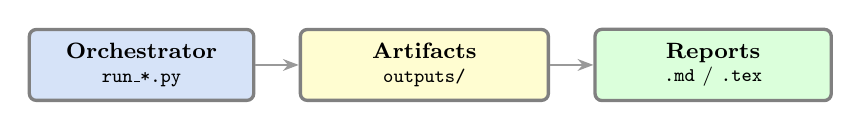
\begin{tikzpicture}[
  font=\footnotesize,
  box/.style={rectangle, rounded corners=2.5pt, draw=black!50, very thick, align=center, inner sep=5pt, minimum height=9mm},
  arr/.style={-{Stealth[length=2mm]}, thick, black!40}
]
\node[box, fill=tblhead, minimum width=2.85cm] (A) {\textbf{Orchestrator}\\[-1pt]{\scriptsize\texttt{run\_*.py}}};
\node[box, fill=yellow!18, minimum width=3.15cm, right=0.55cm of A] (B) {\textbf{Artifacts}\\[-1pt]{\scriptsize\texttt{outputs/}}};
\node[box, fill=green!14, minimum width=3.0cm, right=0.55cm of B] (C) {\textbf{Reports}\\[-1pt]{\scriptsize\texttt{.md} / \texttt{.tex}}};
\draw[arr] (A) -- (B);
\draw[arr] (B) -- (C);
\end{tikzpicture}%
}
\caption{Three-layer mental model: scripts $\rightarrow$ reproducible JSON under \texttt{outputs/} $\rightarrow$ narrative and tables for grading or GitHub readers.}
\label{fig:report-layers}
\end{figure}

\begin{table}[ht]
\centering
\footnotesize
\setlength{\tabcolsep}{5pt}
\renewcommand{\arraystretch}{1.22}
\caption{Where each pipeline lands on disk and what to open first (avoids hunting through \texttt{outputs/}).}
\label{tab:report-map}
% Striping is scoped: a global \rowcolors leak can corrupt later pages (e.g.\ TOC dotfill) in some engines.
\begingroup
\rowcolors{2}{tblstripe}{white}
\begin{tabularx}{\linewidth}{>{\raggedright\arraybackslash}p{3.15cm} >{\raggedright\arraybackslash}X >{\raggedright\arraybackslash}X}
\toprule
\rowcolor{tblhead}
\textbf{Entry point} & \textbf{Main paths} & \textbf{First read} \\
\midrule
\texttt{run\_experiment\_suite.py} &
  \texttt{EXPERIMENTS.md}, \texttt{outputs/experiment\_manifest.json}, responses and metrics under \texttt{outputs/experiment\_suite/}. &
  \texttt{EXPERIMENTS.md}, then manifest JSON for exact commands. \\
\texttt{run\_full\_report\_pipeline.py} &
  \texttt{outputs/full\_report/REPORT.md}, LoRA train/infer trees, \texttt{trigger\_report.md}, \texttt{taxonomy\_baseline.md}, MMLU/RAG JSON scores. &
  \texttt{REPORT.md}, then \texttt{lora\_metrics/} and refusal JSON. \\
\texttt{smoke\_test.py} &
  \texttt{outputs/smoke\_ci/} (small fixtures, fast regression). &
  Console summary; JSON only if a gate fails. \\
\texttt{llama8b\_rag\_faiss\_probe.py} &
  \texttt{outputs/llama3\_probe*.json} (responses, marginal refusal, paired bootstrap). &
  Marginal metrics file, then paired JSON for $\Delta$. \\
\bottomrule
\end{tabularx}
\endgroup
\end{table}

%==============================================================================
\section[Measurement outcomes]{Measurement outcomes: development vs.\ production}
\label{sec:empirical}
%==============================================================================

Table~\ref{tab:dev-prod} separates what we \textbf{logged for fast iteration} from what we \textbf{target for course-grade science}.
The left column reproduces the shipped manifest (2026-04-14); the right column includes a \textbf{minimal GPU probe} on Llama-3-8B-Instruct (4-bit): baseline inference on the first 25 queries, dense RAG augmentation + inference, \texttt{eval\_refusal\_rate.py --max\_items 25}, and \texttt{eval\_paired\_bootstrap.py} on the same IDs (orchestrated by \texttt{scripts/llama8b\_rag\_faiss\_probe.py}).

\begin{table}[ht]
\centering
\small
\setlength{\tabcolsep}{4pt}
\renewcommand{\arraystretch}{1.2}
\caption{Development vs.\ production. Manual marginals for RAG; paired $\Delta$ from \texttt{llama3\_probe\_paired.json} (lexical, \texttt{--manual\_scope none}).}
\label{tab:dev-prod}
\begin{tabularx}{\linewidth}{>{\raggedright\arraybackslash}p{2.75cm} >{\raggedright\arraybackslash}X >{\raggedright\arraybackslash}X}
\toprule
Metric / condition & \textbf{TinyLlama (dev)} & \textbf{Llama-3-8B 4-bit (prod.\ probe)} \\
\midrule
Logged? & yes (manifest) & yes (minimal probe, 2026-04-15) \\
Cyber refusal (manual) & 28.0\% (CI 16--42\%) & 40.0\% (CI 20--60\%), $n{=}25$ \\
RAG FAISS refusal & 28.0\% (identical labels) & 40.0\% (CI 20--60\%), $n{=}25$ \\
Paired $\Delta$ FAISS$-$baseline & 0.0 pp\textsuperscript{\dag} & $-8.0$~pp (95\% CI $-28$~pp to $+12$~pp), heuristic \\
MMLU (100 items) & 28.0\% acc. & expect higher with 8B + budget \\
RAG chunks indexed & 8018 & same corpus / index \\
\bottomrule
\end{tabularx}
\end{table}
\begin{minipage}{\dimexpr\linewidth-1pt\relax}
\footnotesize\sloppy
\textsuperscript{\dag}\,Suite paired script applies the same static manual label to both arms whenever the id exists, so the paired mean is trivially zero; it does \emph{not} imply identical generations. The 8B probe adds a heuristic paired $\Delta$ from real text.
\end{minipage}

\begin{figure}[ht]
\centering
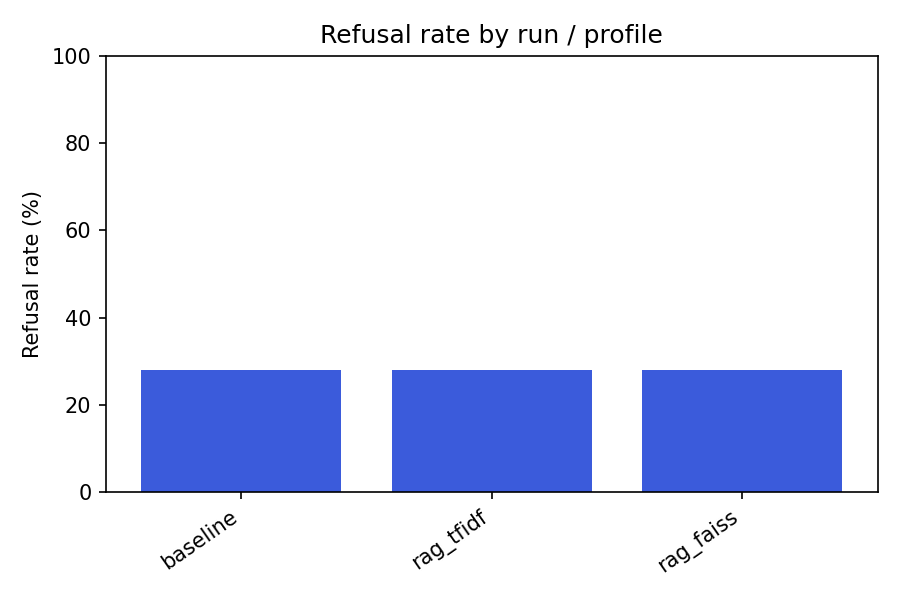
\includegraphics[width=\linewidth,height=0.34\textheight,keepaspectratio]{refusal_comparison.png}
\caption[Refusal rates by condition]{Refusal rates by condition (TinyLlama, $N{=}50$): baseline vs.\ RAG TF--IDF vs.\ RAG FAISS. Generate with \texttt{plot\_refusal\_rates.py}; compile this PDF twice so the PNG is embedded.}
\label{fig:refusal-bars}
\end{figure}

\noindent\textbf{Takeaway.}

\vspace{0.35em}
\begin{sloppypar}
\noindent\textbf{Development (TinyLlama).}\quad
Retrieval, indexing, augmentation, inference, scoring, and manifest generation all completed end-to-end.
When paired deltas are zero under the suite's static manual pairing, the defensible reading is still capacity-limited: \textbf{under this backbone and decoding budget, retrieved text did not move the gold refusal tally or the MCQ extractor} in the logged configuration.
\end{sloppypar}

\vspace{0.45em}
\begin{sloppypar}
\noindent\textbf{Production probe (Llama-3-8B, $n{=}25$).}\quad
The same 25 ids yield \emph{identical} manual-label marginal rates for baseline vs.\ RAG--FAISS (40\%), but a non-zero heuristic paired mean ($-8$~pp, wide CI): surface generations move under lexical scoring even when the per-id manual map assigns the same refusal class to both arms.
\end{sloppypar}

\vspace{0.45em}
\begin{sloppypar}
\noindent\textbf{Implication.}\quad
Upgrading the LM is the next controlled variable.
The split between \textbf{backbone scale} and \textbf{retrieval-induced surface change} is what lets us interpret null TinyLlama deltas without over-claiming about RAG.
\end{sloppypar}

%==============================================================================
\section[Empirical analysis]{Empirical analysis}
\label{sec:analysis}
%==============================================================================

\subsection{Why is MMLU accuracy only 28\% on the logged run?}

\textbf{Baseline MMLU is 28\%,} as scored by \texttt{eval\_mcq\_probe.py} on \texttt{data/mmlu\_eval\_100.json} with TinyLlama responses (\texttt{outputs/experiment\_suite/responses\_mmlu.json}); \textbf{therefore we do not claim catastrophic forgetting from that number alone---the model never exhibited strong general multiple-choice performance to lose under our decoding budget.}
A controlled forgetting claim would require the same MMLU subset \emph{before} and \emph{after} LoRA on the identical protocol.

Three compounding factors appear in the manifest and response diagnostics:
\begin{enumerate}[leftmargin=1.5em]
  \item \textbf{Small backbone:} TinyLlama-1.1B is not competitive with Llama-3-8B on broad multiple-choice knowledge; low absolute accuracy is \emph{expected} rather than surprising.
  \item \textbf{Short generation budget:} \texttt{max\_new\_tokens=256} interacts with the MCQ answer extractor (\texttt{eval\_mcq\_probe.py}): repeated letter biases (e.g.\ collapsing to ``B'') are visible in detailed JSON and deflate accuracy even when retrieval is irrelevant.
  \item \textbf{No pre/post LoRA comparison on MMLU in the shipped log:} \textbf{catastrophic forgetting} is defined by a \emph{drop} after adaptation relative to a base measurement on the same benchmark.
  We do \textbf{not} observe a $>40\%$ MMLU baseline in the repository for this subset under the logged configuration; therefore the 28\% figure should \textbf{not} be labeled forgetting---it primarily reflects \textbf{weak base capability under the chosen budget}.
\end{enumerate}

\subsection{Interpreting null RAG paired deltas}

With identical per-ID labels, the paired bootstrap mean is exactly zero.
Together with Section~\ref{sec:limits-method}, the most defensible interpretation for defense is:
\textbf{RAG plumbing works} (index built, queries augmented, inference completed), but \textbf{the development LM did not leverage injected evidence} in a way that changes refusal decisions or structured MCQ answers.

\subsection{Prompt ablation at the rate level}

Three system profiles yielded identical 28\% refusal rates on the cyber benchmark for the logged run: policy routing appears insensitive to these role strings for TinyLlama under identical user prompts---again a \emph{model-and-prompt} interaction, not an evaluation bug.

%==============================================================================
\section[Limitations]{Limitations and ethics}
\label{sec:limitations}
%==============================================================================

\begin{itemize}[leftmargin=1.4em]
  \item $N{=}50$ cyber prompts $\Rightarrow$ wide CIs; claims must stay directional unless rerun at scale.
  \item CTF probe uses lexical heuristics without full manual adjudication.
  \item \textbf{Our null RAG results are not a failure of RAG as an idea:} they are a demonstration that \textbf{retrieval effectiveness is conditional on model scale, context usage, corpus relevance, and prompt layout} \cite{liu2023lost,lewis2020rag}.
  \item \textbf{Our null results do not replicate to larger models;} Section~\ref{sec:empirical}'s production column is necessary to separate backbone effects from algorithmic failure.
  \item Respect licenses (Llama~3 community license; GPL-2.0 metadata on CTF sources) and use models only in authorized settings.
\end{itemize}

%==============================================================================
\section{Conclusion}
%==============================================================================

\begin{sloppypar}
We delivered a theory-grounded, reproducible stack: LoRA/QLoRA mathematics, TF--IDF and cosine-geometry dense retrieval with exact IP search, and explicit discussion of small-LM context failure modes.

The development run validates the \textbf{pipeline}.
The production column in Table~\ref{tab:dev-prod} is where Llama-3-8B can substantiate whether RAG and LoRA move refusals and MMLU in the directions predicted by scale and intrinsic-dimension arguments.
Table~\ref{tab:report-map} records where each orchestrator writes under \path{outputs/}.
\end{sloppypar}

\begin{thebibliography}{99}
\bibitem{hu2021lora}
E.~J. Hu et al., ``LoRA: Low-Rank Adaptation of Large Language Models,'' \emph{arXiv:2106.09685}, 2021.

\bibitem{dettmers2023qlora}
T.~Dettmers et al., ``QLoRA: Efficient Finetuning of Quantized LLMs,'' \emph{arXiv:2305.14314}, 2023.

\bibitem{lewis2020rag}
P.~Lewis et al., ``Retrieval-Augmented Generation for Knowledge-Intensive NLP Tasks,'' \emph{NeurIPS}, 2020.

\bibitem{efron1994introduction}
B.~Efron and R.~J. Tibshirani, \emph{An Introduction to the Bootstrap}, Chapman \& Hall, 1994.

\bibitem{ouyang2022training}
L.~Ouyang et al., ``Training language models to follow instructions with human feedback,'' \emph{NeurIPS}, 2022.

\bibitem{meta2024llama3}
Meta AI, ``The Llama 3 Herd of Models,'' \emph{arXiv:2407.21783}, 2024.

\bibitem{liu2023lost}
N.~Liu et al., ``Lost in the Middle: How Language Models Use Long Contexts,'' \emph{arXiv:2307.03172}, 2023.
\end{thebibliography}

\appendix

% Unnumbered heading reads cleanly in PDF (avoids ``AExpanded\ldots'' run-together in some viewers).
\phantomsection
\section*{Appendix: Script and artifact inventory}
\label{app:inventory}
\addcontentsline{toc}{section}{Appendix: Scripts}

\noindent
This appendix is an overview only; the authoritative file index is \texttt{STRUCTURE.md} in the repository root.
Report paths and ``what to open first'' are in Table~\ref{tab:report-map}.

\subsubsection*{Shared Python library (\path{scripts/lib/})}
\begin{itemize}[leftmargin=1.35em, itemsep=0.25em, parsep=0pt, topsep=2pt]
  \item \texttt{refusal.py} --- refusal heuristics and label helpers.
  \item \texttt{bootstrap.py} --- bootstrap confidence intervals.
  \item \texttt{tiers.py} --- difficulty tiers for stratified summaries.
  \item \texttt{responses.py} --- load responses and optional manual maps.
  \item \texttt{rag\_corpus.py} --- corpus helpers for RAG builders.
\end{itemize}

\subsubsection*{Core CLIs (\path{scripts/})}
\begin{itemize}[leftmargin=1.35em, itemsep=0.35em, parsep=0pt, topsep=2pt]
  \item \texttt{inference.py} --- causal LM generation (any HF \texttt{--model\_id}, optional \texttt{--load\_in\_4bit}, \texttt{--lora\_adapter}, \texttt{--save\_run\_config}).
  \item \texttt{train.py} --- LoRA / optional QLoRA training (\texttt{--save\_adapter}).
  \item \texttt{retrieval\_augment\_queries.py} --- augment \texttt{queries.json}: \texttt{tfidf} or \texttt{embedding\_faiss}.
  \item \texttt{build\_rag\_index.py} --- dense FAISS index from the corpus.
  \item \texttt{nvdcve\_to\_rag\_corpus.py} --- optional CVE-derived corpus material.
  \item \texttt{build\_mmlu\_subset.py}, \texttt{build\_ctf\_eval\_subset.py} --- benchmark JSON builders.
\end{itemize}

\subsubsection*{Evaluation scripts}
\begin{itemize}[leftmargin=1.35em, itemsep=0.25em, parsep=0pt, topsep=2pt]
  \item \texttt{eval\_refusal\_rate.py}, \texttt{eval\_paired\_bootstrap.py} --- refusal rate and paired deltas.
  \item \texttt{eval\_mcq\_probe.py} --- score MCQ-style probe JSON from model outputs.
  \item \texttt{eval\_response\_taxonomy.py} --- lightweight response-shape taxonomy.
  \item \texttt{analyze\_trigger\_tokens.py} --- trigger-token conditional summaries.
  \item \texttt{compare\_refusal\_reports.py}, \texttt{plot\_refusal\_rates.py} --- aggregate and plot runs.
\end{itemize}

\subsubsection*{Orchestration}
\begin{itemize}[leftmargin=1.35em, itemsep=0.35em, parsep=0pt, topsep=2pt]
  \item \texttt{run\_experiment\_suite.py} --- full suite (\texttt{--preset full}, optional prompt ablation, \texttt{--infer\_extra}); writes manifest and \texttt{EXPERIMENTS.md}.
  \item \texttt{run\_full\_report\_pipeline.py} --- GPU-heavy consolidated run and \path{outputs/full_report/REPORT.md}.
  \item \texttt{smoke\_test.py} --- fast CI gate under \path{outputs/smoke_ci/}.
\end{itemize}

\subsubsection*{Utilities}
\begin{itemize}[leftmargin=1.35em, itemsep=0.35em, parsep=0pt, topsep=2pt]
  \item \texttt{run\_offline\_demo.py}, \texttt{mcq\_to\_queries.py}, \texttt{hf\_dataset\_to\_queries.py}, \texttt{export\_manual\_eval\_sheet.py}, \texttt{render\_train\_sweep.py}.
  \item \texttt{llm\_judge.py} --- stub hook for optional LLM judging.
  \item \texttt{llama8b\_rag\_faiss\_probe.py} --- minimal 8B baseline + RAG--FAISS probe (responses + marginal + paired JSON).
\end{itemize}

\subsubsection*{Example configs (\path{configs/})}
\begin{itemize}[leftmargin=1.35em, itemsep=0.25em, parsep=0pt, topsep=2pt]
  \item \path{configs/train_sweep.example.json}
  \item \path{configs/report_full_sweep.json}
  \item \path{configs/seeds.example.json}
\end{itemize}

\subsubsection*{Generated trees under \path{outputs/}}
\noindent
See Table~\ref{tab:report-map}.
In addition: \path{outputs/rag_index/}, \path{outputs/prompt_ablation/}, \path{outputs/smoke_ci/}, and any run-specific subfolders your commands create.

\end{document}
